% ============================================================================
% Capítulo 6. Resultados
% Requiere \usepackage{graphicx} y \usepackage{booktabs} en el preámbulo.
% Las tablas ya están dentro de este archivo, cada una con su \label{tab:CODIGO}.
% Las figuras se leen de la carpeta figuras/.
% ============================================================================

\chapter{Resultados}
\label{cap:resultados}

Este capítulo presenta primero la composición del catálogo y las muestras empleadas. Después se examina la información aportada por la masa y la metalicidad estelar en tres niveles: el régimen de radio de los planetas, la masa de planetas pequeños a radio comparable y la arquitectura observada de los sistemas multiplanetarios. El análisis de super-Tierras y sub-Neptunos profundiza en la transición entre dos regímenes de planetas pequeños.

\section{Descripción del catálogo y de las muestras}
\label{sec:res-catalogo}

\subsection{Composición del catálogo}
\label{sec:res-catalogo-composicion}

El catálogo descargado contenía 6\,324 planetas confirmados. Tras excluir los 57 que el archivo marca como controversiales, el catálogo depurado quedó en 6\,267 planetas alrededor de 4\,711 estrellas anfitrionas. El 74.4\,\% de esos planetas se descubrió por tránsito y el 18.5\,\% por velocidad radial. La Tabla~\ref{tab:D-T3} resume la distribución de las principales propiedades planetarias y estelares. El planeta mediano tiene un radio de 2.85~$R_\oplus$ y un período orbital de 10.6~días, y la estrella anfitriona mediana, 0.94~$M_\odot$ y una metalicidad cercana a la solar. La masa planetaria, el período y el semieje mayor abarcan varios órdenes de magnitud, lo que justifica trabajar en escala logarítmica con variables como el período orbital, el flujo incidente, el radio y la masa planetaria. El desglose de los registros descartados y la composición por método de descubrimiento se presentan en el anexo.

\begin{table}[htbp]
    \centering
    \caption{Estadística descriptiva de las variables planetarias y estelares principales.}
    \label{tab:D-T3}
    \small
    \resizebox{\textwidth}{!}{%
    \begin{tabular}{llrrrrrrr}
    \toprule
    Variable & Unidad & $N$ & Mediana & $Q_1$ & $Q_3$ & IQR & Mín. & Máx. \\
    \midrule
    $R_p$ & radios terrestres & 6\,223 & 2.850 & 1.840 & 11.900 & 10.060 & 0.310 & 87.206 \\
    $M_p$ & masas terrestres & 6\,241 & 9.220 & 4.300 & 184.3 & 180.0 & 0.020 & 9534.9 \\
    $\bar\rho$ & g/cm$^{3}$ & 6\,199 & 2.584 & 1.325 & 4.627 & 3.302 & 0.030 & 13870.9 \\
    $P$ & días & 5\,927 & 10.641 & 4.300 & 37.574 & 33.274 & 0.091 & $4.02\times10^{8}$ \\
    $a$ & au & 5\,846 & 0.102 & 0.052 & 0.302 & 0.250 & 0.004 & 19000.0 \\
    $T_{\rm eff}$ & K & 5\,970 & 5544.0 & 4901.5 & 5897.0 & 995.5 & 415.0 & 29564.0 \\
    $M_\star$ & masas solares & 6\,260 & 0.940 & 0.770 & 1.084 & 0.314 & 0.009 & 9.100 \\
    $R_\star$ & radios solares & 5\,953 & 0.952 & 0.770 & 1.242 & 0.472 & 0.012 & 88.475 \\
    {[Fe/H]} & dex & 5\,639 & 0.020 & -0.080 & 0.130 & 0.210 & -1.000 & 0.790 \\
    Edad & Gyr & 4\,853 & 3.990 & 2.310 & 5.690 & 3.380 & 0.000 & 16.100 \\
    Distancia & pc & 6\,240 & 364.0 & 102.5 & 826.3 & 723.7 & 1.301 & 8500.0 \\
    \bottomrule
    \end{tabular}
    }
    \par\smallskip
    {\footnotesize\textit{Nota:} Incluye radios y masas estimados por el archivo para planetas sin medición directa.}
\end{table}

\subsection{Disponibilidad y procedencia de los parámetros}
\label{sec:res-catalogo-parametros}

La disponibilidad de parámetros no fue uniforme: las medidas necesarias para clasificar planetas por radio estuvieron presentes en una población más amplia que las requeridas para estudiar simultáneamente masa, radio, irradiación y propiedades estelares. Entre los predictores, la metalicidad fue el menos completo, disponible para el 90.0\,\% de los planetas. Por ello, cada análisis utiliza una submuestra distinta. Las variables seleccionadas y sus fracciones de datos disponibles se detallan en el anexo.

Un valor disponible, además, no siempre es una medición. La tabla de parámetros compuestos completa los radios y las masas que faltan con una relación masa--radio: de los 6\,223 planetas con radio, 4\,701 se observaron en tránsito, y solo en 2\,390 la masa catalogada es una masa verdadera. Por esta razón los análisis~I y~II se apoyan en planetas de tránsito, y el análisis~II exige además una masa verdadera.

La distribución de radios de la Figura~\ref{fig:D-F3} permite ubicar los regímenes empleados en el análisis~I, cuyos tamaños en el catálogo completo se resumen en la Tabla~\ref{tab:D-T5}. Entre los gigantes gaseosos, solo 752 de 1\,853 se observaron en tránsito; los radios estimados del resto producen la acumulación alrededor de 13~$R_\oplus$ que se aprecia en el panel (a). El diagrama masa--radio de la Figura~\ref{fig:D-F4}, construido con los 1\,504 planetas de tránsito que tienen masa verdadera, muestra la dispersión de masas a radios comparables y ofrece el contexto observacional del análisis~II. La densidad calculada a partir de masa y radio se utilizó para la descripción de los planetas, pero no se trató como una medición independiente de ambas variables.

\begin{table}[htbp]
    \centering
    \caption{Regímenes de radio en el catálogo limpio: criterio, número de planetas y medianas de las propiedades planetarias y estelares.}
    \label{tab:D-T5}
    \small
    \resizebox{\textwidth}{!}{%
    \begin{tabular}{llrrrrrrrr}
    \toprule
    Régimen & Criterio & $N_{\rm pl}$ & \% & $N_\star$ & En tránsito & $R_p$ med. & $P$ med. & $M_\star$ med. & {[Fe/H]} med. \\
    \midrule
    Terrestre & $R_p$ $<$ 1.25 $R_\oplus$ & 571 & 9.2 & 473 & 533 & 1.05 & 4.55 & 0.832 & -0.020 \\
    Super-Tierra & 1.25 $\leq$ $R_p$ $<$ 2 $R_\oplus$ & 1\,188 & 19.1 & 1\,023 & 1\,125 & 1.59 & 6.45 & 0.890 & 0.000 \\
    Tipo Neptuno & 2 $\leq$ $R_p$ $<$ 6 $R_\oplus$ & 2\,374 & 38.1 & 1\,904 & 2\,075 & 2.72 & 14.15 & 0.920 & 0.010 \\
    Gigante gaseoso & 6 $\leq$ $R_p$ $<$ 15 $R_\oplus$ & 1\,853 & 29.8 & 1\,645 & 752 & 12.70 & 85.33 & 1.030 & 0.100 \\
    Mayor que Júpiter & $R_p$ $\geq$ 15 $R_\oplus$ & 237 & 3.8 & 235 & 216 & 16.81 & 3.31 & 1.300 & 0.050 \\
    \bottomrule
    \end{tabular}
    }
    \par\smallskip
    {\footnotesize\textit{Nota:} 44 planetas no tienen radio. Los planetas que no transitan tienen radios estimados por el archivo.}
\end{table}

\begin{figure}[htbp]
\centering
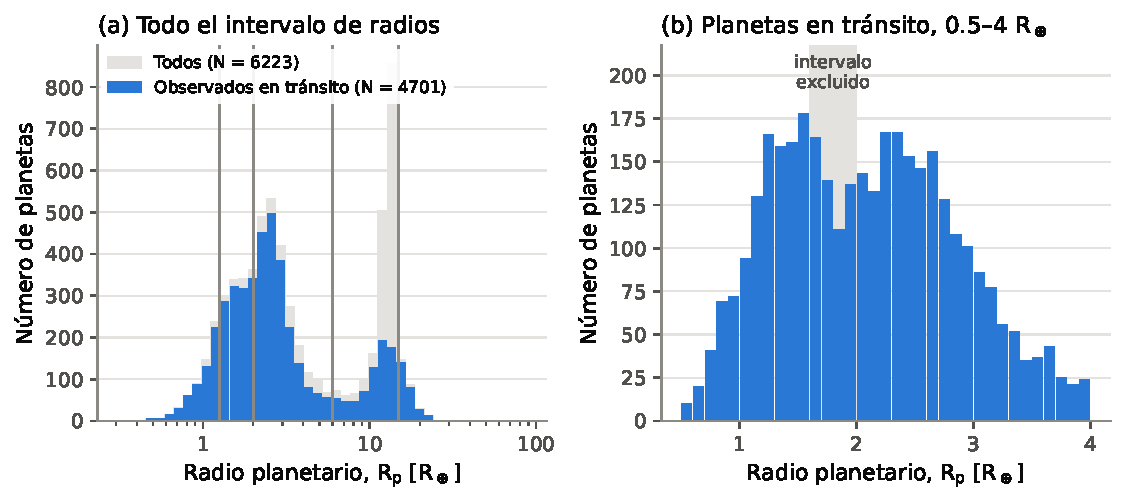
\includegraphics[width=\textwidth]{figuras/D-F3_distribucion_radio_planetario}
\caption{Distribución del radio planetario. (a) Todo el catálogo; las líneas verticales marcan los límites de los cinco regímenes (1.25, 2, 6 y 15~$R_\oplus$). (b) Planetas en tránsito entre 0.5 y 4~$R_\oplus$; la banda gris marca el intervalo 1.6--2.0~$R_\oplus$ excluido en el análisis de super-Tierras y sub-Neptunos.}
\label{fig:D-F3}
\end{figure}

\begin{figure}[htbp]
\centering
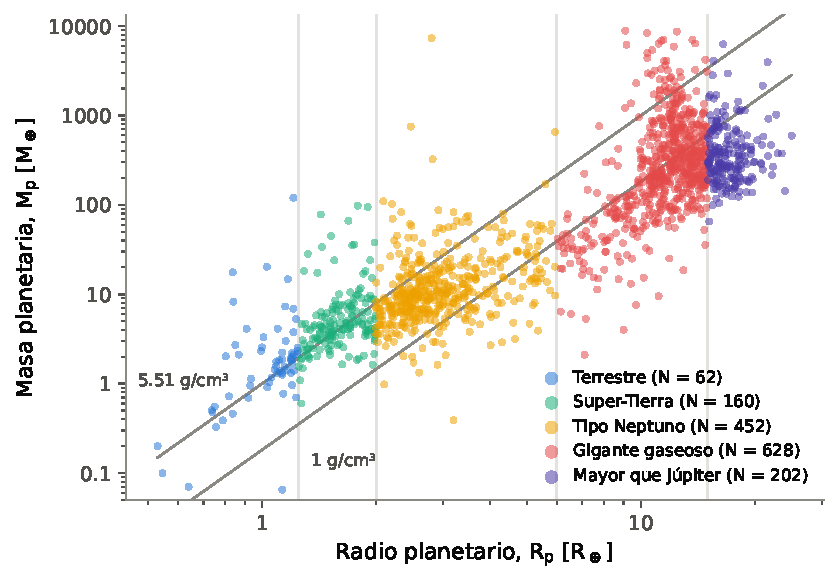
\includegraphics[width=0.82\textwidth]{figuras/D-F4_diagrama_masa_radio}
\caption{Diagrama masa--radio de los planetas en tránsito con masa verdadera, por régimen de radio. Las curvas grises son líneas de densidad constante (1 y 5.51~g/cm$^{3}$).}
\label{fig:D-F4}
\end{figure}

\subsection{Submuestras analíticas}
\label{sec:res-submuestras}

Los requisitos de cada respuesta determinaron el tamaño final de las submuestras (Tabla~\ref{tab:D-T8}). El modelo general de regímenes de radio utilizó 4\,461 planetas en tránsito alrededor de 3\,390 estrellas. El análisis enfocado en super-Tierras y sub-Neptunos reunió 2\,565 planetas alrededor de 1\,981 estrellas. El estudio de la masa de planetas pequeños quedó restringido a 574 planetas alrededor de 385 estrellas, mientras que el análisis de arquitectura comprendió 615 sistemas multiplanetarios con 1\,513 planetas. Estos tamaños corresponden a unidades de observación y requisitos de disponibilidad diferentes; por ello, no se interpretan como etapas sucesivas de una única muestra. Tampoco son muestras independientes: la de super-Tierras y sub-Neptunos está contenida en la del análisis~I, a la que pertenecen también 550 de los 574 planetas del análisis~II y 1\,359 de los 1\,513 del análisis~III.

\begin{table}[htbp]
    \centering
    \caption{Submuestras utilizadas en los tres análisis.}
    \label{tab:D-T8}
    \small
    \resizebox{\textwidth}{!}{%
    \begin{tabular}{llp{0.40\textwidth}rr}
    \toprule
    Análisis & Unidad & Criterios de selección & $N_{\rm pl}$ & $N_\star$ \\
    \midrule
    I. Regímenes de radio & Planeta & Descubiertos por tránsito, con radio, período, masa estelar y metalicidad & 4\,461 & 3\,390 \\
    I. Super-Tierras y sub-Neptunos & Planeta & Tránsito, 1--4 $R_\oplus$ excluyendo 1.6--2.0 $R_\oplus$, con flujo incidente, masa estelar y metalicidad & 2\,565 & 1\,981 \\
    II. Propiedades físicas & Planeta & 1--4 $R_\oplus$, masa verdadera y radio medido sin límites, flujo incidente, masa estelar y metalicidad & 574 & 385 \\
    III. Arquitectura & Sistema & Al menos 2 planetas de 1--4 $R_\oplus$ y $P$ $<$ 100 d, con masa estelar y metalicidad & 1\,513 & 615 \\
    \bottomrule
    \end{tabular}
    }
    \par\smallskip
    {\footnotesize\textit{Nota:} En el análisis III cada estrella es un sistema; el número de planetas es el total en esos sistemas.}
\end{table}

\section{Análisis I: regímenes de radio}
\label{sec:res-analisis-I}

\subsection{Propiedades estelares por régimen de radio}
\label{sec:res-regimenes-descripcion}

De los 4\,461 planetas de la muestra en tránsito, 514 se clasificaron como terrestres, 1\,080 como super-Tierras, 1\,937 como planetas de tipo Neptuno, 720 como gigantes gaseosos y 210 como mayores que Júpiter (Tabla~\ref{tab:A1-T1}). La Figura~\ref{fig:A1-F1} muestra la distribución de masa y metalicidad de las estrellas anfitrionas en cada régimen. La mediana de la masa estelar aumenta con el tamaño del planeta, de 0.86~$M_\odot$ en los terrestres a 1.32~$M_\odot$ en los mayores que Júpiter, y la metalicidad mediana es más alta en los gigantes gaseosos (0.12~dex) que en los tres regímenes de menor tamaño, donde es prácticamente solar. Las pruebas de Kruskal--Wallis y las comparaciones por pares, que confirman que ambas propiedades difieren entre regímenes, se presentan en el anexo. Estas diferencias descriptivas motivan el análisis multivariable posterior: por sí solas no establecen cuánto aportan las propiedades estelares después de considerar el período orbital.

\begin{table}[htbp]
    \centering
    \caption{Análisis I: composición de la muestra de planetas en tránsito por régimen de radio.}
    \label{tab:A1-T1}
    \small
    \resizebox{\textwidth}{!}{%
    \begin{tabular}{llrrrrr}
    \toprule
    Régimen & Criterio & $N_{\rm pl}$ & \% & $P$ med. [d] & $M_\star$ med. [$M_\odot$] & {[Fe/H]} med. \\
    \midrule
    Terrestre & $R_p$ $<$ 1.25 $R_\oplus$ & 514 & 11.5 & 4.46 & 0.860 & -0.010 \\
    Super-Tierra & 1.25 $\leq$ $R_p$ $<$ 2 $R_\oplus$ & 1\,080 & 24.2 & 6.50 & 0.910 & 0.000 \\
    Tipo Neptuno & 2 $\leq$ $R_p$ $<$ 6 $R_\oplus$ & 1\,937 & 43.4 & 14.55 & 0.939 & 0.010 \\
    Gigante gaseoso & 6 $\leq$ $R_p$ $<$ 15 $R_\oplus$ & 720 & 16.1 & 4.62 & 1.034 & 0.120 \\
    Mayor que Júpiter & $R_p$ $\geq$ 15 $R_\oplus$ & 210 & 4.7 & 3.28 & 1.322 & 0.064 \\
    \bottomrule
    \end{tabular}
    }
    \par\smallskip
    {\footnotesize\textit{Nota:} N = 4461 planetas alrededor de 3390 estrellas.}
\end{table}

\begin{figure}[htbp]
\centering
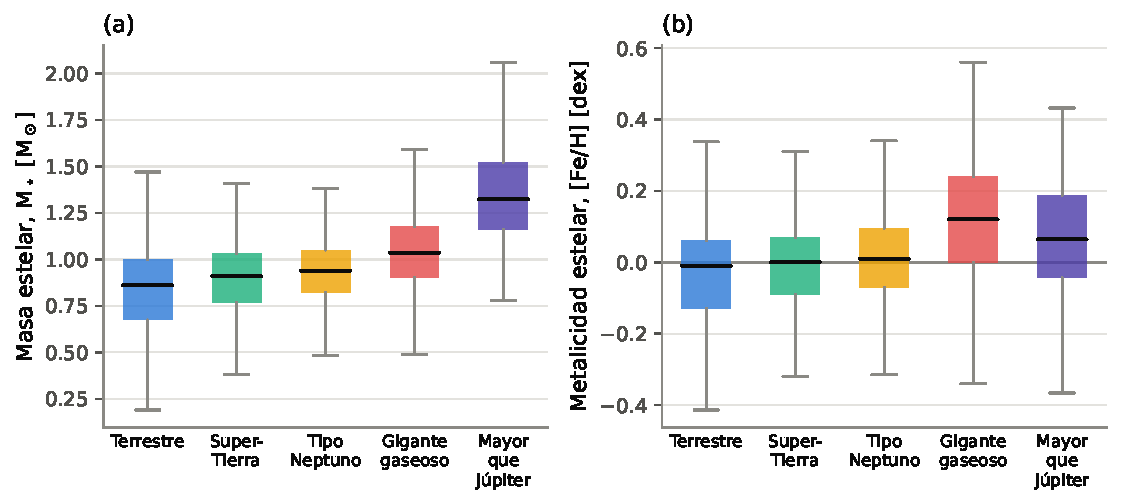
\includegraphics[width=\textwidth]{figuras/A1-F1_propiedades_estelares_por_regimen}
\caption{Distribución de (a) la masa estelar y (b) la metalicidad de las estrellas anfitrionas por régimen de radio. Las cajas muestran la mediana y los cuartiles; los bigotes, 1.5 veces el rango intercuartílico.}
\label{fig:A1-F1}
\end{figure}

\subsection{Modelo multinomial de cinco regímenes}
\label{sec:res-multinomial}

Al añadir masa y metalicidad estelar al modelo basado en el período orbital, el AIC disminuyó de 11\,548.1 a 10\,480.6 y el pseudo-$R^2$ de McFadden aumentó de 0.0720 a 0.1592 (Tabla~\ref{tab:A1-T4}). El log-loss en la muestra de ajuste disminuyó de 1.2925 a 1.1711. La masa estelar por sí sola produjo una mejora mayor que la metalicidad por sí sola (reducción del AIC de 825.4 frente a 368.5). En conjunto, las propiedades estelares añadieron información para distinguir las cinco clases dentro de la muestra analizada.

\begin{table}[htbp]
    \centering
    \caption{Análisis I: comparación de los modelos multinomiales. Las diferencias son respecto al modelo base B0.}
    \label{tab:A1-T4}
    \small
    \resizebox{\textwidth}{!}{%
    \begin{tabular}{llrrrrrrrrr}
    \toprule
    Modelo & Predictores & $N_\star$ & $N_{\rm pl}$ & pseudo-$R^2$ & AIC & BIC & log-loss & $\Delta$AIC & $\Delta$pseudo-$R^2$ & $\Delta$log-loss \\
    \midrule
    B0 & $\log P$ & 3\,390 & 4\,461 & 0.0720 & 11548.1 & 11599.3 & 1.2925 & +0.0 & +0.0000 & +0.0000 \\
    BM & $\log P$ + $M_\star$ & 3\,390 & 4\,461 & 0.1391 & 10722.7 & 10799.5 & 1.1991 & -825.4 & +0.0671 & -0.0934 \\
    BZ & $\log P$ + {[Fe/H]} & 3\,390 & 4\,461 & 0.1023 & 11179.6 & 11256.4 & 1.2503 & -368.5 & +0.0303 & -0.0422 \\
    B1 & $\log P$ + $M_\star$ + {[Fe/H]} & 3\,390 & 4\,461 & 0.1592 & 10480.6 & 10583.0 & 1.1711 & -1067.5 & +0.0872 & -0.1214 \\
    \bottomrule
    \end{tabular}
    }
    \par\smallskip
    {\footnotesize\textit{Nota:} Métricas calculadas en la muestra de ajuste. pseudo-R2 de McFadden.}
\end{table}

Los coeficientes del modelo estelar se presentan en la Tabla~\ref{tab:A1-T5}, con la super-Tierra como categoría de referencia y los predictores estandarizados. La asociación no fue igual para todos los regímenes: la masa estelar mostró una relación particularmente marcada con las clases de gigantes gaseosos y planetas mayores que Júpiter en comparación con las super-Tierras. Por cada desviación estándar adicional de masa estelar, la razón de riesgo relativo fue de 1.86 (IC del 95\,\%: $[1.64, 2.10]$) para los gigantes gaseosos y de 8.88 ($[7.01, 11.25]$) para los mayores que Júpiter. La metalicidad se asoció con los gigantes gaseosos (2.15; $[1.92, 2.40]$) y, en menor medida, con los planetas de tipo Neptuno (1.26; $[1.16, 1.37]$), pero no con los mayores que Júpiter (0.89; $[0.72, 1.09]$). Para los planetas terrestres, ambas razones fueron menores que uno. La interpretación de estos coeficientes es relativa a la categoría de referencia y se complementa más adelante con probabilidades predichas. Los errores estándar de este modelo no están agrupados por estrella.

\begin{table}[htbp]
    \centering
    \caption{Análisis I: coeficientes del modelo multinomial estelar B1, respecto al régimen de super-Tierra. Predictores estandarizados.}
    \label{tab:A1-T5}
    \small
    \resizebox{\textwidth}{!}{%
    \begin{tabular}{llrrrrrrrr}
    \toprule
    Régimen & Predictor & Coef. & EE & IC 95\,\% inf. & IC 95\,\% sup. & $p$ & RRR & RRR inf. & RRR sup. \\
    \midrule
    Terrestre & $\log P$ & -0.501 & 0.068 & -0.633 & -0.369 & $<0.001$ & 0.606 & 0.531 & 0.692 \\
    Terrestre & $M_\star$ & -0.182 & 0.061 & -0.301 & -0.063 & 0.003 & 0.834 & 0.740 & 0.939 \\
    Terrestre & {[Fe/H]} & -0.139 & 0.055 & -0.247 & -0.030 & 0.012 & 0.871 & 0.781 & 0.970 \\
    Tipo Neptuno & $\log P$ & 0.836 & 0.048 & 0.742 & 0.930 & $<0.001$ & 2.307 & 2.100 & 2.534 \\
    Tipo Neptuno & $M_\star$ & 0.083 & 0.048 & -0.011 & 0.177 & 0.082 & 1.087 & 0.990 & 1.194 \\
    Tipo Neptuno & {[Fe/H]} & 0.230 & 0.043 & 0.145 & 0.314 & $<0.001$ & 1.258 & 1.156 & 1.369 \\
    Gigante gaseoso & $\log P$ & 0.265 & 0.060 & 0.148 & 0.382 & $<0.001$ & 1.303 & 1.159 & 1.465 \\
    Gigante gaseoso & $M_\star$ & 0.621 & 0.063 & 0.497 & 0.744 & $<0.001$ & 1.860 & 1.645 & 2.104 \\
    Gigante gaseoso & {[Fe/H]} & 0.764 & 0.058 & 0.650 & 0.877 & $<0.001$ & 2.146 & 1.915 & 2.405 \\
    Mayor que Júpiter & $\log P$ & -1.601 & 0.152 & -1.898 & -1.303 & $<0.001$ & 0.202 & 0.150 & 0.272 \\
    Mayor que Júpiter & $M_\star$ & 2.184 & 0.121 & 1.947 & 2.421 & $<0.001$ & 8.880 & 7.008 & 11.252 \\
    Mayor que Júpiter & {[Fe/H]} & -0.122 & 0.108 & -0.333 & 0.089 & 0.258 & 0.885 & 0.717 & 1.093 \\
    \bottomrule
    \end{tabular}
    }
    \par\smallskip
    {\footnotesize\textit{Nota:} RRR: razón de riesgo relativo, exp(coeficiente). Intervalos de confianza al 95 \%.}
\end{table}

\subsection{Contribución de la masa estelar y de la metalicidad por régimen}
\label{sec:res-contribucion-regimen}

La mejora del modelo no se distribuyó uniformemente entre las clases (Tabla~\ref{tab:A1-T6}; Figura~\ref{fig:A1-F2}). La comparación se hizo con el log-loss medio de los planetas observados en cada régimen. Al añadir únicamente la masa estelar al modelo base, la reducción del log-loss fue de 0.099 para los planetas terrestres, 0.043 para las super-Tierras, 0.011 para los de tipo Neptuno, 0.088 para los gigantes gaseosos y 1.113 para los mayores que Júpiter. Al añadir únicamente la metalicidad, la reducción mayor correspondió a los gigantes gaseosos (0.152). En el resto de las clases, la reducción asociada con la masa estelar fue mayor que la asociada con la metalicidad.

\begin{table}[htbp]
    \centering
    \caption{Análisis I: reducción del log-loss de cada régimen al añadir la masa estelar, la metalicidad o ambas al modelo base.}
    \label{tab:A1-T6}
    \small
    \resizebox{\textwidth}{!}{%
    \begin{tabular}{lrrrrrrrlrr}
    \toprule
    Régimen & $N_{\rm pl}$ & log-loss B0 & Gan. $M_\star$ & Gan. {[Fe/H]} & Gan. ambas & $M_\star \mid$ {[Fe/H]} & {[Fe/H]} $\mid M_\star$ & Dominante & AUC B0 & AUC B1 \\
    \midrule
    Terrestre & 514 & 1.963 & 0.099 & 0.077 & 0.136 & 0.059 & 0.038 & $M_\star$ & 0.689 & 0.749 \\
    Super-Tierra & 1\,080 & 1.387 & 0.043 & 0.029 & 0.060 & 0.030 & 0.016 & $M_\star$ & 0.568 & 0.646 \\
    Tipo Neptuno & 1\,937 & 0.715 & 0.011 & 0.003 & 0.015 & 0.012 & 0.004 & $M_\star$ & 0.744 & 0.751 \\
    Gigante gaseoso & 720 & 1.857 & 0.088 & 0.152 & 0.192 & 0.039 & 0.103 & {[Fe/H]} & 0.546 & 0.699 \\
    Mayor que Júpiter & 210 & 2.560 & 1.113 & 0.007 & 1.144 & 1.137 & 0.031 & $M_\star$ & 0.812 & 0.945 \\
    \bottomrule
    \end{tabular}
    }
    \par\smallskip
    {\footnotesize\textit{Nota:} Ganancia = log-loss de B0 menos log-loss del modelo ampliado, entre los planetas del régimen. AUC de cada régimen frente al resto (descriptivo).}
\end{table}

\begin{figure}[htbp]
\centering
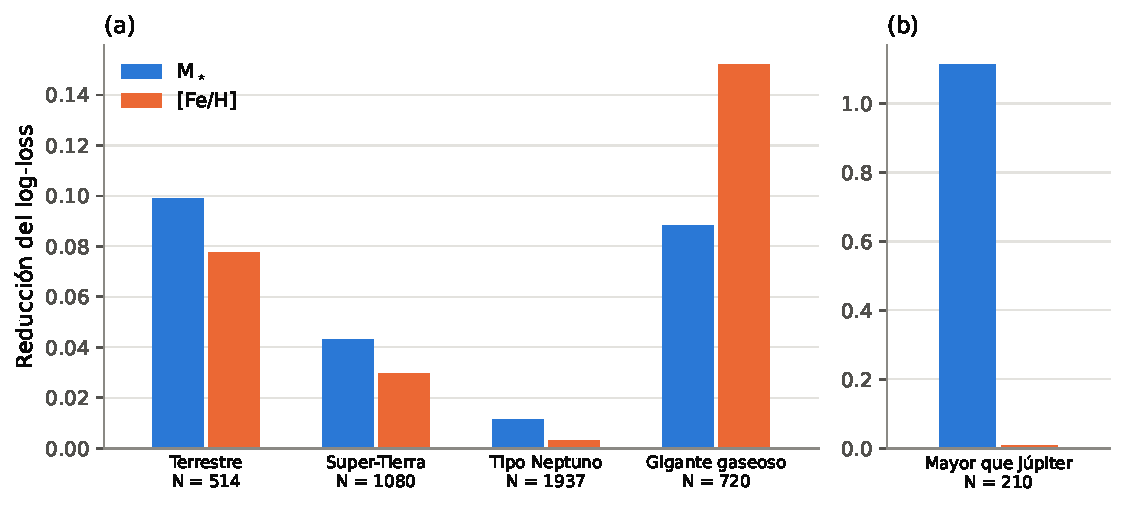
\includegraphics[width=\textwidth]{figuras/A1-F2_ganancia_de_informacion_por_regimen}
\caption{Reducción del log-loss de cada régimen de radio al añadir al modelo base la masa estelar o la metalicidad. (a) Regímenes de terrestre a gigante gaseoso. (b) Planetas mayores que Júpiter, en escala propia. Resultados calculados en la muestra de ajuste.}
\label{fig:A1-F2}
\end{figure}

Las probabilidades predichas de la Figura~\ref{fig:A1-F3} permiten visualizar cómo cambia la composición esperada de los regímenes al variar la masa estelar o la metalicidad, manteniendo el período orbital y la otra propiedad estelar en su mediana. Entre los percentiles 20 y 80 de la masa estelar (0.78 y 1.11~$M_\odot$), la probabilidad predicha de gigante gaseoso pasa de 0.11 a 0.21; entre los mismos percentiles de la metalicidad ($-0.10$ y 0.14~dex), de 0.11 a 0.23. Tanto la comparación por clase como estas probabilidades proceden del modelo ajustado a la muestra disponible. En particular, la reducción de log-loss para la clase mayor que Júpiter debe leerse teniendo presente que contiene 210 planetas y que esta comparación no se validó fuera de muestra.

\begin{figure}[htbp]
\centering
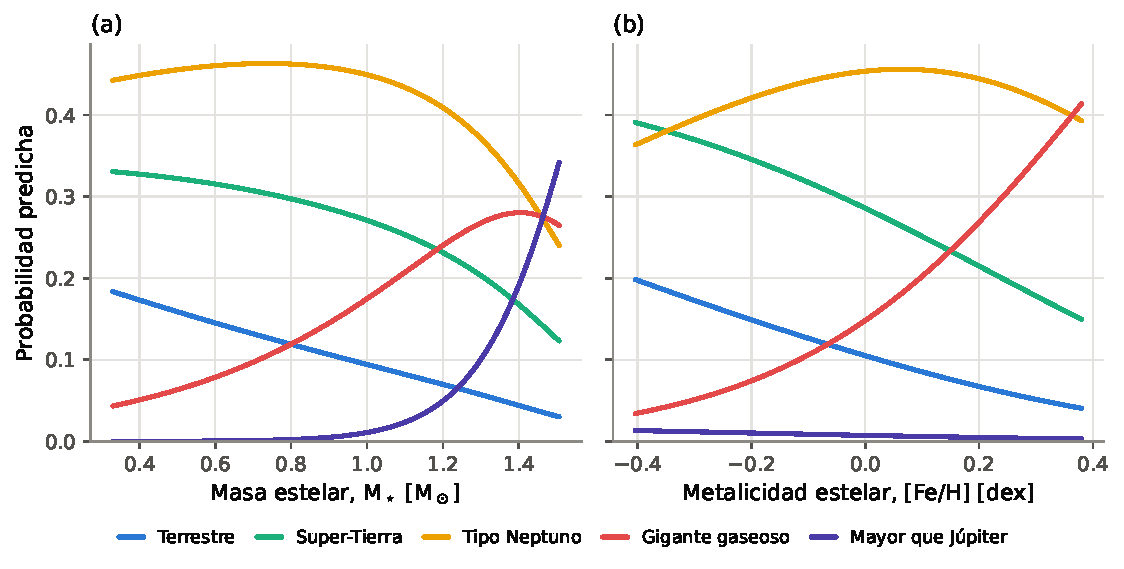
\includegraphics[width=\textwidth]{figuras/A1-F3_probabilidades_predichas_por_regimen}
\caption{Probabilidad predicha de cada régimen de radio según el modelo multinomial B1, en función de (a) la masa estelar y (b) la metalicidad. El período orbital y la otra propiedad estelar se fijan en su mediana.}
\label{fig:A1-F3}
\end{figure}

\subsection{Verificación con el radio como variable continua}
\label{sec:res-radio-continuo}

El radio planetario se examinó también como respuesta continua para comprobar si la asociación observada en la clasificación multinomial dependía de los límites entre categorías. La Tabla~\ref{tab:A1-T8} presenta el ajuste de esta verificación y, en su nota, los coeficientes estelares. Al añadir masa y metalicidad estelar, el $R^2$ aumentó de 0.066 a 0.227 y el AIC disminuyó en 843.6. Ambos coeficientes fueron positivos: 0.123~dex por desviación estándar de masa estelar (IC del 95\,\%: $[0.112, 0.133]$) y 0.055~dex por desviación estándar de metalicidad ($[0.043, 0.067]$). La comparación con el resultado categórico debe centrarse en la dirección de las asociaciones estelares y en su incertidumbre, ya que ambos modelos representan respuestas distintas. En ese sentido los dos coinciden: los planetas de mayor radio se encuentran alrededor de estrellas más masivas y más ricas en metales, de modo que el resultado multinomial no depende de dónde se trazaron los límites entre regímenes.

\begin{table}[htbp]
    \centering
    \caption{Análisis I: verificación con el radio como variable continua. Respuesta: logaritmo del radio planetario.}
    \label{tab:A1-T8}
    \small
    \resizebox{\textwidth}{!}{%
    \begin{tabular}{llrrrrrrrrrr}
    \toprule
    Modelo & Predictores & $N_{\rm pl}$ & $R^2$ & $R^2_{\rm aj}$ & AIC & BIC & RMSE & MAE & $\Delta R^2$ & $\Delta$AIC & $\Delta$RMSE \\
    \midrule
    C0 & $s($$\log P$$)$ & 4\,461 & 0.066 & 0.065 & 3350.9 & 3389.3 & 0.352 & 0.278 & +0.0000 & +0.0 & +0.0000 \\
    C1 & $s($$\log P$$)$ + $M_\star$ + {[Fe/H]} & 4\,461 & 0.227 & 0.226 & 2507.3 & 2558.5 & 0.320 & 0.254 & +0.1617 & -843.6 & -0.0319 \\
    C2 & $s($$\log P$$)$ + $s($$M_\star$$)$ + $s(${[Fe/H]}$)$ & 4\,461 & 0.265 & 0.262 & 2299.8 & 2389.4 & 0.312 & 0.243 & +0.1988 & -1051.1 & -0.0397 \\
    \bottomrule
    \end{tabular}
    }
    \par\smallskip
    {\footnotesize\textit{Nota:} s() denota un spline cúbico. Coeficientes estandarizados en C1 (IC 95 \%, errores agrupados por estrella): st\_mass\_z: 0.123 [0.112, 0.133]; st\_met\_z: 0.055 [0.043, 0.067].}
\end{table}

\section{Análisis I: super-Tierras y sub-Neptunos}
\label{sec:res-zoom}

\subsection{Fracción de sub-Neptunos según el flujo incidente y la masa estelar}
\label{sec:res-zoom-fracciones}

El análisis enfocado en planetas pequeños partió de los 3\,261 planetas descubiertos por tránsito con radio entre 1 y 4~$R_\oplus$ (Tabla~\ref{tab:Z-T1}): 873 super-Tierras, 1\,820 sub-Neptunos y 568 en el intervalo de $1.6$--$2.0\,R_{\oplus}$, excluido de la comparación binaria. La Figura~\ref{fig:Z-F1} muestra los intervalos de radio utilizados. Con flujo incidente, masa estelar y metalicidad disponibles, la muestra de los modelos quedó en 2\,565 planetas alrededor de 1\,981 estrellas, de los cuales el 66.9\,\% son sub-Neptunos.

\begin{table}[htbp]
    \centering
    \caption{Planetas de 1 a 4 $R_\oplus$: muestra principal (tránsito) y muestras de robustez.}
    \label{tab:Z-T1}
    \small
    \resizebox{\textwidth}{!}{%
    \begin{tabular}{lrrrrrrrr}
    \toprule
    Muestra & $N_{\rm pl}$ & $N_\star$ & Super-Tierras & Excluidos & Sub-Neptunos & $N$ modelo & $N_\star$ modelo & Fracción SN \\
    \midrule
    Tránsito & 3\,261 & 2\,423 & 873 & 568 & 1\,820 & 2\,565 & 1\,981 & 0.669 \\
    Todos los métodos & 3\,592 & 2\,621 & 934 & 613 & 2\,045 & 2\,775 & 2\,097 & 0.678 \\
    Kepler & 2\,300 & 1\,694 & 659 & 424 & 1\,217 & 1\,876 & 1\,455 & 0.649 \\
    \bottomrule
    \end{tabular}
    }
    \par\smallskip
    {\footnotesize\textit{Nota:} N modelo: planetas clasificados (fuera del intervalo 1.6--2.0 $R_\oplus$) con flujo incidente, masa estelar y metalicidad.}
\end{table}

\begin{figure}[htbp]
\centering
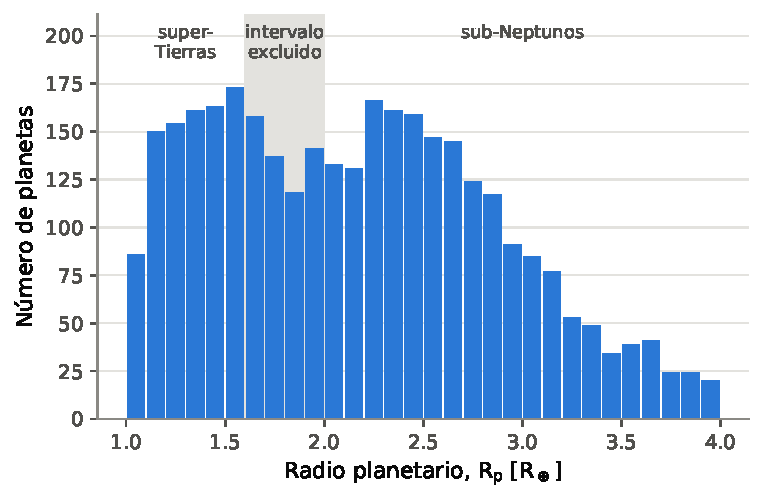
\includegraphics[width=0.78\textwidth]{figuras/Z-F1_distribucion_radios_planetas_pequenos}
\caption{Distribución de radios de los planetas en tránsito entre 1 y 4~$R_\oplus$ y clasificación conservadora: super-Tierras (1--1.6~$R_\oplus$), intervalo excluido (1.6--2.0~$R_\oplus$) y sub-Neptunos (2--4~$R_\oplus$).}
\label{fig:Z-F1}
\end{figure}

La fracción observada de sub-Neptunos varió con el flujo incidente y con la masa de la estrella anfitriona (Tabla~\ref{tab:Z-T2}; Figura~\ref{fig:Z-F2}). En términos generales, la fracción subneptuniana disminuyó hacia irradiaciones mayores: pasó de 0.80 en el cuartil de menor flujo a 0.43 en el de mayor flujo. Con la masa estelar ocurrió lo contrario: la fracción fue de 0.58 en el tercil de menor masa y de 0.72 y 0.71 en los otros dos. La distribución por grupos sirve como descripción inicial; la comparación de modelos de la siguiente subsección evalúa si las propiedades estelares aportan información una vez incluida la irradiación.

\begin{table}[htbp]
    \centering
    \caption{Fracción observada de sub-Neptunos por cuartil de flujo incidente y por tercil de masa estelar, con intervalo de Wilson al 95 \%.}
    \label{tab:Z-T2}
    \small
    \resizebox{\textwidth}{!}{%
    \begin{tabular}{llrrrrrrrr}
    \toprule
    Variable & Grupo & Mín. & Mediana & Máx. & $N$ & Sub-Neptunos & Fracción & IC 95\,\% inf. & IC 95\,\% sup. \\
    \midrule
    $\log F$ & C1 (bajo) & -0.845 & 0.933 & 1.308 & 642 & 511 & 0.796 & 0.763 & 0.825 \\
    $\log F$ & C2 & 1.309 & 1.604 & 1.850 & 641 & 507 & 0.791 & 0.758 & 0.821 \\
    $\log F$ & C3 & 1.851 & 2.096 & 2.345 & 641 & 421 & 0.657 & 0.619 & 0.693 \\
    $\log F$ & C4 (alto) & 2.345 & 2.642 & 4.100 & 641 & 278 & 0.434 & 0.396 & 0.472 \\
    $M_\star$ & T1 (baja) & 0.090 & 0.730 & 0.840 & 855 & 492 & 0.575 & 0.542 & 0.608 \\
    $M_\star$ & T2 & 0.841 & 0.920 & 0.990 & 862 & 619 & 0.718 & 0.687 & 0.747 \\
    $M_\star$ & T3 (alta) & 0.990 & 1.087 & 2.018 & 848 & 606 & 0.715 & 0.683 & 0.744 \\
    \bottomrule
    \end{tabular}
    }
\end{table}

\begin{figure}[htbp]
\centering
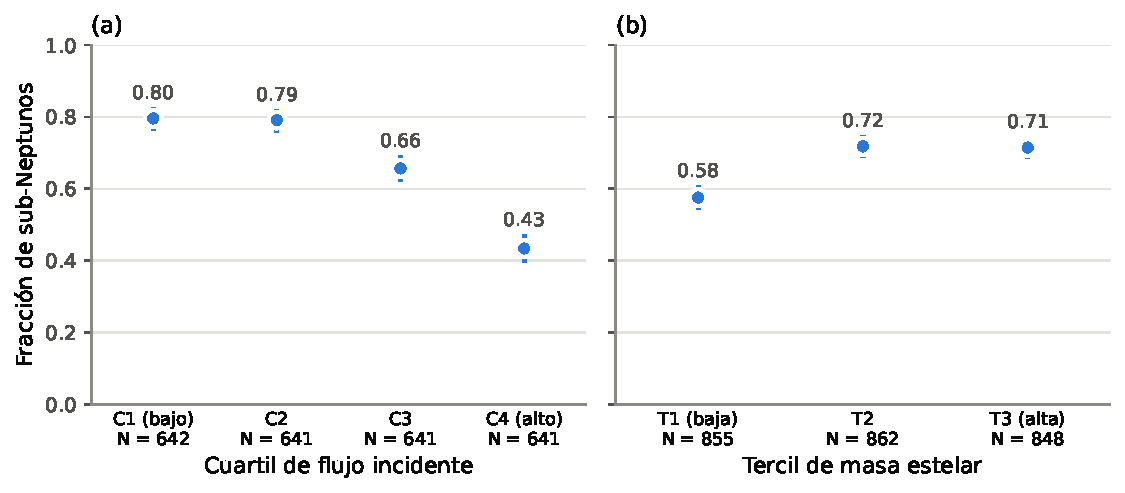
\includegraphics[width=\textwidth]{figuras/Z-F2_fraccion_sub_neptunos_por_flujo_y_masa_estelar}
\caption{Fracción observada de sub-Neptunos (a) por cuartil de flujo incidente y (b) por tercil de masa estelar. Las barras verticales son intervalos de Wilson al 95\,\%.}
\label{fig:Z-F2}
\end{figure}

\subsection{Modelos logísticos y contribución estelar}
\label{sec:res-zoom-modelos}

Se comparó un modelo basado en irradiación ($M_0$), uno que añadió masa y metalicidad estelar ($M_1$) y otro que incorporó además la interacción entre flujo y masa estelar ($M_2$). La Tabla~\ref{tab:Z-T3} reúne sus métricas de ajuste. Al pasar de $M_0$ a $M_1$, el pseudo-$R^2$ de McFadden aumentó de 0.074 a 0.178 y el AIC disminuyó en 336.5. La mejora del modelo al incorporar propiedades estelares se mantuvo en la validación cruzada agrupada por estrella (Tabla~\ref{tab:Z-T5}): el log-loss disminuyó de 0.589 en $M_0$ a 0.523 en $M_1$, y el Brier score de 0.199 a 0.174.

\begin{table}[htbp]
    \centering
    \caption{Super-Tierras y sub-Neptunos: comparación de los modelos logísticos en la muestra de ajuste. Diferencias respecto a M0.}
    \label{tab:Z-T3}
    \small
    \resizebox{\textwidth}{!}{%
    \begin{tabular}{llrrrrrrrrrr}
    \toprule
    Modelo & Predictores & $N_{\rm pl}$ & pseudo-$R^2$ & AIC & BIC & log-loss & Brier & $\Delta$AIC & $\Delta$pseudo-$R^2$ & $\Delta$log-loss & $\Delta$Brier \\
    \midrule
    M0 & $\log F$ & 2\,565 & 0.074 & 3019.1 & 3030.8 & 0.588 & 0.199 & +0.0 & 0.000 & 0.000 & 0.000 \\
    M1 & $\log F$ + $M_\star$ + {[Fe/H]} & 2\,565 & 0.178 & 2682.6 & 2706.0 & 0.521 & 0.174 & -336.5 & 0.105 & -0.066 & -0.025 \\
    M2 & $\log F$ + $M_\star$ + {[Fe/H]} + $\log F \times M_\star$ & 2\,565 & 0.191 & 2642.4 & 2671.6 & 0.513 & 0.171 & -376.7 & 0.118 & -0.075 & -0.028 \\
    \bottomrule
    \end{tabular}
    }
    \par\smallskip
    {\footnotesize\textit{Nota:} 2565 planetas alrededor de 1981 estrellas. pseudo-R2 de McFadden.}
\end{table}

\begin{table}[htbp]
    \centering
    \caption{Super-Tierras y sub-Neptunos: desempeño en validación cruzada de cinco pliegues agrupada por estrella. Diferencias respecto a M0.}
    \label{tab:Z-T5}
    \small
    \begin{tabular}{lrrrrrr}
    \toprule
    Modelo & log-loss VC & D.E. & Brier VC & D.E. & $\Delta$log-loss & $\Delta$Brier \\
    \midrule
    M0 & 0.589 & 0.017 & 0.199 & 0.008 & 0.000 & 0.000 \\
    M1 & 0.523 & 0.025 & 0.174 & 0.011 & -0.066 & -0.025 \\
    M2 & 0.515 & 0.029 & 0.172 & 0.012 & -0.073 & -0.027 \\
    \bottomrule
    \end{tabular}
    \par\smallskip
    {\footnotesize\textit{Nota:} Media y desviación estándar entre pliegues.}
\end{table}

Las razones de momios de la Tabla~\ref{tab:Z-T7} cuantifican las asociaciones estimadas por los modelos logísticos. En $M_1$, un aumento de 1~dex en el flujo incidente multiplicó los momios de ser sub-Neptuno por 0.18 (IC del 95\,\%: $[0.15, 0.21]$), mientras que un aumento de 0.1~$M_\odot$ en la masa estelar los multiplicó por 1.54 ($[1.45, 1.64]$) y un aumento de 0.1~dex en la metalicidad, por 1.09 ($[1.02, 1.16]$). En el modelo con interacción, la asociación del flujo con la clasificación no se representa mediante una sola razón de momios válida para todas las masas estelares; su valor depende de $M_\star$. Por ello se presentan también efectos del flujo calculados para masas estelares representativas.

\begin{table}[htbp]
    \centering
    \caption{Super-Tierras y sub-Neptunos: razones de momios de ser sub-Neptuno por incrementos físicos y por una desviación estándar de cada predictor.}
    \label{tab:Z-T7}
    \small
    \resizebox{\textwidth}{!}{%
    \begin{tabular}{lllrrrr}
    \toprule
    Modelo & Predictor & Incremento & OR & OR inf. & OR sup. & $p$ \\
    \midrule
    M1 & $\log F$ & +1 dex & 0.177 & 0.146 & 0.214 & $<0.001$ \\
    M1 & $M_\star$ & +0.1 $M_\odot$ & 1.541 & 1.452 & 1.635 & $<0.001$ \\
    M1 & {[Fe/H]} & +0.1 dex & 1.087 & 1.018 & 1.161 & 0.013 \\
    M1 & $\log F$ & +1 DE (0.76 dex) & 0.270 & 0.234 & 0.311 & $<0.001$ \\
    M1 & $M_\star$ & +1 DE (0.23 $M_\odot$) & 2.671 & 2.334 & 3.057 & $<0.001$ \\
    M1 & {[Fe/H]} & +1 DE (0.16 dex) & 1.144 & 1.029 & 1.271 & 0.013 \\
    M2 & $\log F$ & +1 dex & 0.163 & 0.134 & 0.197 & $<0.001$ \\
    M2 & $M_\star$ & +0.1 $M_\odot$ & 1.515 & 1.431 & 1.603 & $<0.001$ \\
    M2 & {[Fe/H]} & +0.1 dex & 1.105 & 1.035 & 1.180 & 0.003 \\
    M2 & $\log F$ & +1 DE (0.76 dex) & 0.253 & 0.219 & 0.293 & $<0.001$ \\
    M2 & $M_\star$ & +1 DE (0.23 $M_\odot$) & 2.568 & 2.258 & 2.920 & $<0.001$ \\
    M2 & {[Fe/H]} & +1 DE (0.16 dex) & 1.174 & 1.057 & 1.304 & 0.003 \\
    \bottomrule
    \end{tabular}
    }
    \par\smallskip
    {\footnotesize\textit{Nota:} En M2 los efectos de log F y de la masa estelar corresponden al valor medio de la otra variable. DE: desviación estándar.}
\end{table}

\subsection{Interacción entre el flujo incidente y la masa estelar}
\label{sec:res-zoom-interaccion}

El modelo con interacción mejoró el ajuste frente a $M_1$: el AIC disminuyó de 2\,682.6 a 2\,642.4 y el pseudo-$R^2$ de McFadden aumentó de 0.178 a 0.191. La mejora también se mantuvo fuera de muestra: en validación cruzada agrupada, el log-loss disminuyó de 0.523 a 0.515 y el Brier score de 0.174 a 0.172. El coeficiente estimado para la interacción fue negativo ($\beta=-1.590$; IC del 95\,\%: $[-2.127,-1.054]$).

La Tabla~\ref{tab:Z-T8} expresa el efecto del flujo para tres valores representativos de masa estelar. La razón de momios por cada dex de flujo fue de 0.20 para una estrella de 0.76~$M_\odot$, de 0.16 para una de 0.92~$M_\odot$ y de 0.13 para una de 1.06~$M_\odot$. Las curvas de la Figura~\ref{fig:Z-F3} muestran la consecuencia en la escala de probabilidad: la relación estimada entre irradiación y pertenencia al grupo subneptuniano cambia de pendiente con $M_\star$ y es más pronunciada alrededor de estrellas más masivas. Así, la interacción aporta una descripción que el modelo de efectos únicamente aditivos no reproduce.

\begin{table}[htbp]
    \centering
    \caption{Efecto del flujo incidente sobre los momios de ser sub-Neptuno para tres masas estelares (modelo M2).}
    \label{tab:Z-T8}
    \small
    \resizebox{\textwidth}{!}{%
    \begin{tabular}{lrrrrrrr}
    \toprule
    Percentil & $M_\star$ [$M_\odot$] & Pendiente & IC 95\,\% inf. & IC 95\,\% sup. & OR & OR inf. & OR sup. \\
    \midrule
    P20 & 0.760 & -1.592 & -1.786 & -1.399 & 0.203 & 0.168 & 0.247 \\
    P50 & 0.920 & -1.847 & -2.041 & -1.652 & 0.158 & 0.130 & 0.192 \\
    P80 & 1.063 & -2.075 & -2.299 & -1.850 & 0.126 & 0.100 & 0.157 \\
    \bottomrule
    \end{tabular}
    }
    \par\smallskip
    {\footnotesize\textit{Nota:} OR por cada aumento de 1 dex en el flujo incidente.}
\end{table}

\begin{figure}[htbp]
\centering
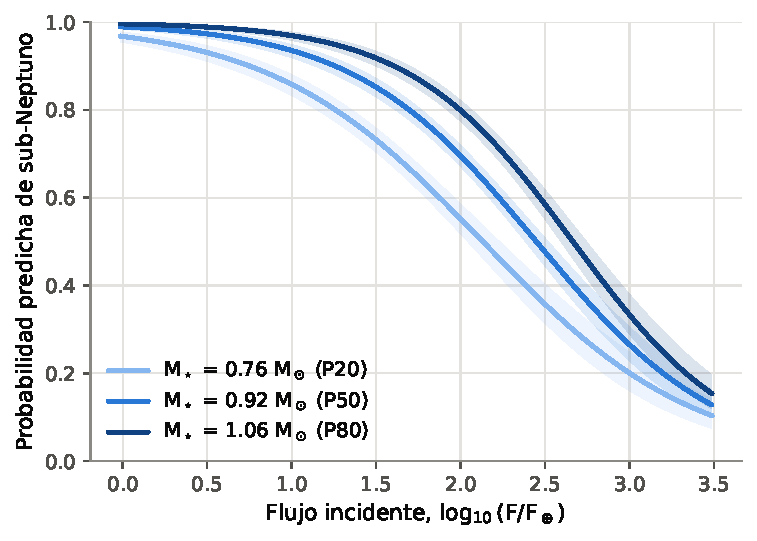
\includegraphics[width=0.78\textwidth]{figuras/Z-F3_probabilidad_sub_neptuno_vs_flujo}
\caption{Probabilidad predicha de que un planeta de 1--4~$R_\oplus$ sea sub-Neptuno en función del flujo incidente, para tres masas estelares (percentiles 20, 50 y 80). Modelo $M_2$ con la metalicidad fija en la mediana; las bandas son intervalos de confianza al 95\,\%.}
\label{fig:Z-F3}
\end{figure}

\subsection{Verificaciones de robustez}
\label{sec:res-zoom-robustez}

La interacción se evaluó nuevamente con otras tres definiciones de la muestra (Tabla~\ref{tab:Z-T11}): los planetas de todos los métodos de descubrimiento, los planetas asociados con Kepler y la muestra de tránsito con un corte único en 1.6~$R_\oplus$, sin excluir el intervalo de 1.6--2.0~$R_\oplus$. Los coeficientes recuperados conservaron el signo negativo: $-1.496$, $-2.018$ y $-1.281$, respectivamente, y en los tres casos el intervalo de confianza excluye el cero. Esta coincidencia respalda que la interacción del modelo principal no depende del método de descubrimiento ni de la exclusión del intervalo intermedio, aunque su magnitud varía entre muestras.

\begin{table}[htbp]
    \centering
    \caption{Robustez de la interacción entre flujo incidente y masa estelar: coeficiente en M2 y mejora de M2 respecto a M1 en distintas muestras y definiciones.}
    \label{tab:Z-T11}
    \small
    \resizebox{\textwidth}{!}{%
    \begin{tabular}{lrrrrrrrrr}
    \toprule
    Variante & $N_{\rm pl}$ & $N_\star$ & Coef. interacción & IC 95\,\% inf. & IC 95\,\% sup. & $p$ & $\Delta$AIC & $\Delta$BIC & $\Delta$pseudo-$R^2$ \\
    \midrule
    Tránsito (principal) & 2\,565 & 1\,981 & -1.590 & -2.127 & -1.054 & $<0.001$ & -40.2 & -34.3 & +0.0130 \\
    Todos los métodos & 2\,775 & 2\,097 & -1.496 & -1.908 & -1.084 & $<0.001$ & -53.3 & -47.3 & +0.0158 \\
    Kepler & 1\,876 & 1\,455 & -2.018 & -2.870 & -1.165 & $<0.001$ & -28.6 & -23.1 & +0.0126 \\
    Tránsito, corte único en 1.6 $R_\oplus$ & 3\,116 & 2\,293 & -1.281 & -1.735 & -0.826 & $<0.001$ & -33.0 & -27.0 & +0.0095 \\
    \bottomrule
    \end{tabular}
    }
    \par\smallskip
    {\footnotesize\textit{Nota:} Errores estándar agrupados por estrella.}
\end{table}

Una segunda comprobación sustituyó el flujo incidente por el período orbital como control. Con el período, el modelo $M_1$ ajustó mejor (AIC de 2\,644.3 frente a 2\,682.6; anexo). El flujo incidente se conservó en el modelo principal por su interpretación física, no porque produzca el mejor ajuste.

\section{Análisis II: propiedades físicas de planetas pequeños}
\label{sec:res-analisis-II}

\subsection{Relación masa--radio--irradiación}
\label{sec:res-masa-radio}

La aplicación de los requisitos de radio medido en tránsito, masa verdadera, flujo incidente y propiedades estelares dejó 574 planetas pequeños alrededor de 385 estrellas (Tabla~\ref{tab:A2-T1}). La Figura~\ref{fig:A2-F1} muestra una dispersión considerable de masas a radio comparable. Al representar $\log M_p$ mediante una función spline de $\log R_p$, el modelo basado solo en radio obtuvo $R^2=0.270$ y un RMSE de 0.373~dex en la muestra de ajuste. Esta dispersión motivó evaluar si la irradiación y las propiedades estelares aportaban información adicional.

\begin{table}[htbp]
    \centering
    \caption{Análisis II: construcción de la muestra. Número de planetas y de estrellas después de cada corte sucesivo sobre el catálogo limpio.}
    \label{tab:A2-T1}
    \small
    \begin{tabular}{lrr}
    \toprule
    Corte & $N_{\rm pl}$ & $N_\star$ \\
    \midrule
    Masa y radio disponibles & 6\,199 & 4\,676 \\
    Sin límites superiores o inferiores & 6\,013 & 4\,598 \\
    Solo masa verdadera (\texttt{pl\_bmassprov = Mass}) & 2\,165 & 1\,793 \\
    Radio medido (planeta observado en tránsito) & 1\,504 & 1\,224 \\
    Con masa estelar & 1\,504 & 1\,224 \\
    Con metalicidad & 1\,488 & 1\,208 \\
    Con flujo incidente calculado & 1\,488 & 1\,208 \\
    Planetas pequeños (1 $<$ $R_p$ $<$ 4) & 574 & 385 \\
    \bottomrule
    \end{tabular}
    \par\smallskip
    {\footnotesize\textit{Nota:} Composición final por régimen de radio: terrestre 41, super-tierra 160, tipo neptuno 373.}
\end{table}

\begin{figure}[htbp]
\centering
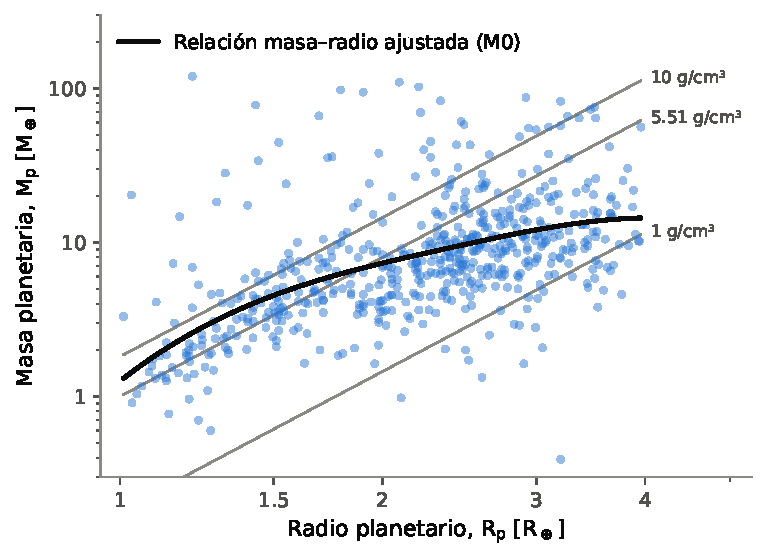
\includegraphics[width=0.78\textwidth]{figuras/A2-F1_diagrama_masa_radio_planetas_pequenos}
\caption{Diagrama masa--radio de la muestra del análisis~II. La curva negra es la relación ajustada con el spline del modelo $M_0$; las líneas grises son curvas de densidad constante.}
\label{fig:A2-F1}
\end{figure}

\subsection{Contribución de las propiedades estelares}
\label{sec:res-contribucion-estelar}

Al comparar el modelo base con radio e irradiación con el modelo que añadió masa y metalicidad estelar, el AIC disminuyó de 500.4 a 484.7 y el $R^2$ aumentó de 0.281 a 0.305 (Tabla~\ref{tab:A2-T2}). En validación cruzada agrupada por estrella, el RMSE disminuyó de 0.372 a 0.367~dex, el MAE de 0.249 a 0.242~dex y el $R^2$ aumentó de 0.269 a 0.286 (Tabla~\ref{tab:A2-T3}). La ganancia predictiva persistió fuera de muestra, aunque fue pequeña en comparación con la variación entre pliegues: el $R^2$ mejoró en cuatro de los cinco (anexo).

\begin{table}[htbp]
    \centering
    \caption{Análisis II: comparación de los modelos de la masa planetaria en la muestra de ajuste. Diferencias respecto al modelo base M1.}
    \label{tab:A2-T2}
    \small
    \resizebox{\textwidth}{!}{%
    \begin{tabular}{llrrrrrrrrrrr}
    \toprule
    Modelo & Predictores & $N_{\rm pl}$ & $R^2$ & $R^2_{\rm aj}$ & AIC & BIC & RMSE & MAE & $\Delta R^2$ & $\Delta$AIC & $\Delta$RMSE & $\Delta$MAE \\
    \midrule
    M0 & $s($$\log R_p$$)$ & 574 & 0.270 & 0.265 & 506.5 & 528.3 & 0.373 & 0.249 & -0.0102 & +6.1 & +0.0026 & +0.0035 \\
    M1 & $s($$\log R_p$$)$ + $\log F$ & 574 & 0.281 & 0.274 & 500.4 & 526.6 & 0.370 & 0.245 & +0.0000 & +0.0 & +0.0000 & +0.0000 \\
    M2 & $s($$\log R_p$$)$ + $\log F$ + $M_\star$ + {[Fe/H]} & 574 & 0.305 & 0.296 & 484.7 & 519.5 & 0.364 & 0.237 & +0.0243 & -15.8 & -0.0063 & -0.0082 \\
    \bottomrule
    \end{tabular}
    }
    \par\smallskip
    {\footnotesize\textit{Nota:} 574 planetas alrededor de 385 estrellas. s() denota un spline cúbico. RMSE y MAE en dex.}
\end{table}

\begin{table}[htbp]
    \centering
    \caption{Análisis II: desempeño en validación cruzada de cinco pliegues agrupada por estrella. Diferencias respecto al modelo base M1.}
    \label{tab:A2-T3}
    \small
    \resizebox{\textwidth}{!}{%
    \begin{tabular}{lrrrrrrrrr}
    \toprule
    Modelo & $R^2$ VC & D.E. & RMSE VC & D.E. & MAE VC & D.E. & $\Delta R^2$ & $\Delta$RMSE & $\Delta$MAE \\
    \midrule
    M0 & 0.261 & 0.097 & 0.374 & 0.057 & 0.252 & 0.028 & -0.0082 & +0.0021 & +0.0034 \\
    M1 & 0.269 & 0.124 & 0.372 & 0.063 & 0.249 & 0.030 & +0.0000 & +0.0000 & +0.0000 \\
    M2 & 0.286 & 0.129 & 0.367 & 0.065 & 0.242 & 0.031 & +0.0174 & -0.0043 & -0.0062 \\
    \bottomrule
    \end{tabular}
    }
    \par\smallskip
    {\footnotesize\textit{Nota:} Media y desviación estándar entre pliegues.}
\end{table}

En el modelo estelar, el coeficiente de la masa estelar estandarizada fue $0.076$ (IC del 95\,\%: $[0.031,0.121]$; Tabla~\ref{tab:A2-T4}). El coeficiente de metalicidad estandarizada fue $0.030$ (IC del 95\,\%: $[-0.008,0.068]$), compatible con cero. El coeficiente del flujo incidente, que en el modelo base era $0.047$ ($[0.015,0.079]$), se redujo a $-0.003$ ($[-0.045,0.040]$) al incluir las propiedades estelares. La Figura~\ref{fig:A2-F2} presenta estas asociaciones después de considerar el radio y la irradiación. A valores comparables de ambos controles, la masa estelar mostró una asociación positiva y modesta con la masa planetaria; la evidencia correspondiente a la metalicidad fue menos clara.

\begin{table}[htbp]
    \centering
    \caption{Análisis II: coeficientes estandarizados del flujo incidente, la masa estelar y la metalicidad en los modelos M1 y M2.}
    \label{tab:A2-T4}
    \small
    \resizebox{\textwidth}{!}{%
    \begin{tabular}{llrrrrr}
    \toprule
    Modelo & Predictor & Coef. & EE & IC 95\,\% inf. & IC 95\,\% sup. & $p$ \\
    \midrule
    M1 & $\log F$ & 0.047 & 0.016 & 0.015 & 0.079 & 0.004 \\
    M2 & $\log F$ & -0.003 & 0.022 & -0.045 & 0.040 & 0.908 \\
    M2 & $M_\star$ & 0.076 & 0.023 & 0.031 & 0.121 & $<0.001$ \\
    M2 & {[Fe/H]} & 0.030 & 0.020 & -0.008 & 0.068 & 0.125 \\
    \bottomrule
    \end{tabular}
    }
    \par\smallskip
    {\footnotesize\textit{Nota:} Cambio en el logaritmo de la masa planetaria (dex) por una desviación estándar del predictor. Errores estándar agrupados por estrella.}
\end{table}

\begin{figure}[htbp]
\centering
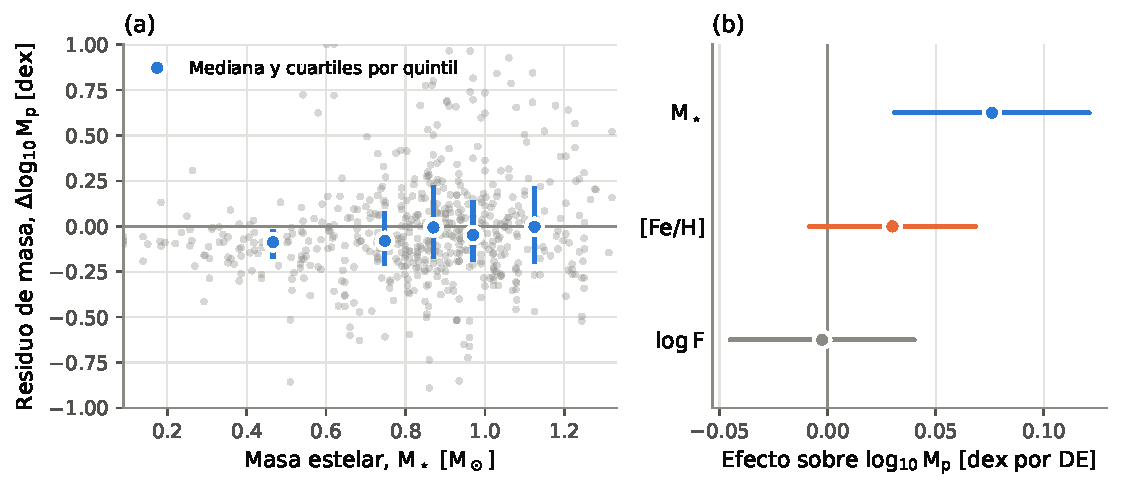
\includegraphics[width=\textwidth]{figuras/A2-F2_efectos_estelares_sobre_la_masa}
\caption{(a) Residuos de masa respecto al modelo base $M_1$ (radio y flujo incidente) en función de la masa estelar; los puntos azules son la mediana y los cuartiles en quintiles de masa estelar. (b) Coeficientes estandarizados del modelo $M_2$ con intervalos de confianza al 95\,\%.}
\label{fig:A2-F2}
\end{figure}

\section{Análisis III: arquitectura de sistemas}
\label{sec:res-analisis-III}

\subsection{Muestra de sistemas multiplanetarios}
\label{sec:res-sistemas-muestra}

La muestra de arquitectura comprendió 615 sistemas y 1\,513 planetas, equivalentes a 898 pares adyacentes observados (Tabla~\ref{tab:A3-T1}). De los sistemas, 415 tenían dos planetas detectados, 137 tenían tres, 47 tenían cuatro y 16 tenían cinco o más. La mediana de la razón de períodos entre planetas adyacentes fue 2.34; la Figura~\ref{fig:A3-F1} sitúa este espaciamiento en relación con la multiplicidad observada. Un total de 85 sistemas (13.8\,\%) cumplió el criterio de sistema \textit{gapped} (Tabla~\ref{tab:A3-T2}). En 542 sistemas (88.1\,\%) todos los planetas se observaron en tránsito; en los 73 restantes interviene al menos un radio estimado.

\begin{table}[htbp]
    \centering
    \caption{Análisis III: construcción de la muestra de sistemas multiplanetarios.}
    \label{tab:A3-T1}
    \small
    \begin{tabular}{p{0.40\textwidth}rr}
    \toprule
    Paso & $N_{\rm pl}$ & $N_\star$ \\
    \midrule
    Catálogo limpio & 6\,267 & 4\,711 \\
    Con radio, período, {[Fe/H]} y masa estelar & 5\,578 & 4\,105 \\
    Radio planetario entre 1 y 4 $R_\oplus$ & 3\,371 & 2\,419 \\
    Período orbital menor que 100 días & 3\,238 & 2\,340 \\
    En sistemas con al menos 2 planetas que cumplen los criterios & 1\,513 & 615 \\
    \bottomrule
    \end{tabular}
    \par\smallskip
    {\footnotesize\textit{Nota:} Las razones de período se calculan solo entre los planetas que cumplen los criterios, ordenados por período.}
\end{table}

\begin{table}[htbp]
    \centering
    \caption{Análisis III: resumen de la muestra de sistemas multiplanetarios.}
    \label{tab:A3-T2}
    \small
    \resizebox{\textwidth}{!}{%
    \begin{tabular}{lp{0.40\textwidth}rr}
    \toprule
     & Característica & Valor & \% \\
    \midrule
    Muestra & Sistemas & 615 & -- \\
    Muestra & Planetas en esos sistemas & 1\,513 & -- \\
    Muestra & Sistemas \textit{gapped} & 85 & 13.8 \\
    Medianas & Mediana de la razón de períodos adyacentes & 2.343 & -- \\
    Medianas & Mediana del radio planetario mediano [$R_\oplus$] & 2.045 & -- \\
    Medianas & Mediana de la masa estelar [$M_\odot$] & 0.885 & -- \\
    Medianas & Mediana de {[Fe/H]} [dex] & -0.006 & -- \\
    Multiplicidad & N = 2 & 415 & 67.5 \\
    Multiplicidad & N = 3 & 137 & 22.3 \\
    Multiplicidad & N = 4 & 47 & 7.6 \\
    Multiplicidad & N $\geq$ 5 & 16 & 2.6 \\
    Origen observacional & Kepler & 389 & 63.3 \\
    Origen observacional & TESS & 95 & 15.4 \\
    Origen observacional & Solo tránsito & 67 & 10.9 \\
    Origen observacional & Velocidad radial & 64 & 10.4 \\
    Radios & Sistemas con todos sus planetas observados en tránsito & 542 & 88.1 \\
    \bottomrule
    \end{tabular}
    }
    \par\smallskip
    {\footnotesize\textit{Nota:} Origen observacional: Kepler o TESS si alguna instalación de descubrimiento lo es; el resto, según el método de detección.}
\end{table}

\begin{figure}[htbp]
\centering
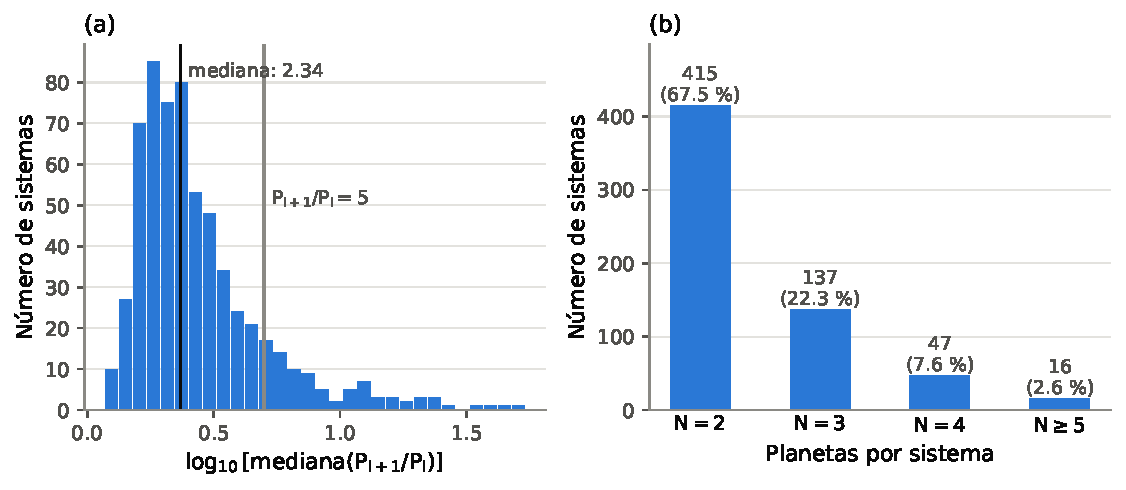
\includegraphics[width=\textwidth]{figuras/A3-F1_panorama_de_la_arquitectura}
\caption{Muestra de sistemas multiplanetarios. (a) Distribución del espaciamiento orbital; la línea negra marca la mediana y la gris, la razón de períodos de 5 que define un sistema \textit{gapped}. (b) Multiplicidad observada.}
\label{fig:A3-F1}
\end{figure}

\subsection{Espaciamiento orbital}
\label{sec:res-espaciamiento}

El modelo que añadió las propiedades estelares explicó una fracción mayor de la variación del espaciamiento que el modelo base: el $R^2$ aumentó de 0.070 a 0.093 y el AIC disminuyó de 50.5 a 39.1 (Tabla~\ref{tab:A3-T5}). El RMSE en la muestra de ajuste disminuyó de 0.251 a 0.248. Estos cambios señalan información adicional en el ajuste, aunque la mayor parte de la variación del espaciamiento permaneció sin explicar.

\begin{table}[htbp]
    \centering
    \caption{Análisis III: comparación de los modelos lineales del espaciamiento orbital. Diferencias respecto al modelo base S0.}
    \label{tab:A3-T5}
    \small
    \resizebox{\textwidth}{!}{%
    \begin{tabular}{lp{0.40\textwidth}rrrrrrrrrrr}
    \toprule
    Modelo & Predictores & $N_{\rm sis}$ & $R^2$ & $R^2_{\rm aj}$ & AIC & BIC & RMSE & MAE & $\Delta R^2$ & $\Delta$AIC & $\Delta$BIC & $\Delta$RMSE \\
    \midrule
    S0 & $\tilde{R}_p$ + $N_{\rm pl}$ & 615 & 0.070 & 0.067 & 50.5 & 63.7 & 0.251 & 0.180 & +0.0000 & +0.0 & +0.0 & +0.0000 \\
    S1 & $\tilde{R}_p$ + $N_{\rm pl}$ + $M_\star$ + {[Fe/H]} & 615 & 0.093 & 0.087 & 39.1 & 61.2 & 0.248 & 0.176 & +0.0229 & -11.3 & -2.5 & -0.0031 \\
    \bottomrule
    \end{tabular}
    }
    \par\smallskip
    {\footnotesize\textit{Nota:} Respuesta: logaritmo decimal de la mediana de las razones de período adyacentes. RMSE y MAE en dex.}
\end{table}

En el modelo estelar, la masa estelar estandarizada se asoció con una menor razón mediana de períodos en escala logarítmica ($\beta=-0.043$; IC del 95\,\%: $[-0.064,-0.021]$; Tabla~\ref{tab:A3-T6}). Para la metalicidad, $\beta=0.015$ (IC del 95\,\%: $[-0.006,0.035]$); este intervalo incluye cero. La asociación con la masa estelar conservó el signo, con menor magnitud, en los 542 sistemas cuyos planetas se observaron todos en tránsito ($\beta=-0.027$; $[-0.050,-0.004]$) y en los 389 sistemas de Kepler ($\beta=-0.025$; $[-0.049,-0.001]$) (anexo). Las asociaciones corresponden al espaciamiento de los planetas detectados, que puede diferir del espaciamiento del sistema completo si faltan planetas por descubrir.

\begin{table}[htbp]
    \centering
    \caption{Análisis III: coeficientes estandarizados del modelo estelar S1 del espaciamiento orbital.}
    \label{tab:A3-T6}
    \small
    \resizebox{\textwidth}{!}{%
    \begin{tabular}{llrrrrr}
    \toprule
    Modelo & Predictor & Coef. & EE & IC 95\,\% inf. & IC 95\,\% sup. & $p$ \\
    \midrule
    S1 & Constante & 0.442 & 0.010 & 0.422 & 0.462 & $<0.001$ \\
    S1 & $\tilde{R}_p$ & 0.027 & 0.011 & 0.006 & 0.048 & 0.011 \\
    S1 & $N_{\rm pl}$ & -0.067 & 0.010 & -0.087 & -0.047 & $<0.001$ \\
    S1 & $M_\star$ & -0.043 & 0.011 & -0.064 & -0.021 & $<0.001$ \\
    S1 & {[Fe/H]} & 0.015 & 0.011 & -0.006 & 0.035 & 0.166 \\
    \bottomrule
    \end{tabular}
    }
    \par\smallskip
    {\footnotesize\textit{Nota:} Cambio en el logaritmo del espaciamiento (dex) por una desviación estándar del predictor.}
\end{table}

\subsection{Sistemas \textit{gapped}}
\label{sec:res-gapped}

Al añadir masa y metalicidad estelar al modelo de clasificación \textit{gapped}, el pseudo-$R^2$ de McFadden aumentó de 0.0184 a 0.0392 y el AIC disminuyó de 491.0 a 484.7 (Tabla~\ref{tab:A3-T7}). En la muestra de ajuste, el log-loss disminuyó de 0.3943 a 0.3860 y el Brier score de 0.1176 a 0.1159. El BIC, que penaliza más los parámetros adicionales, aumentó de 504.3 a 506.8.

\begin{table}[htbp]
    \centering
    \caption{Análisis III: comparación de los modelos logísticos de la condición \textit{gapped}. Diferencias respecto al modelo base G0.}
    \label{tab:A3-T7}
    \small
    \resizebox{\textwidth}{!}{%
    \begin{tabular}{lp{0.40\textwidth}rrrrrrrrrrr}
    \toprule
    Modelo & Predictores & $N_{\rm sis}$ & pseudo-$R^2$ & AIC & BIC & log-loss & Brier & $\Delta$pseudo-$R^2$ & $\Delta$AIC & $\Delta$BIC & $\Delta$log-loss & $\Delta$Brier \\
    \midrule
    G0 & $\tilde{R}_p$ + $N_{\rm pl}$ & 615 & 0.0184 & 491.0 & 504.3 & 0.3943 & 0.1176 & +0.0000 & +0.0 & +0.0 & +0.0000 & +0.0000 \\
    G1 & $\tilde{R}_p$ + $N_{\rm pl}$ + $M_\star$ + {[Fe/H]} & 615 & 0.0392 & 484.7 & 506.8 & 0.3860 & 0.1159 & +0.0208 & -6.3 & +2.6 & -0.0084 & -0.0018 \\
    \bottomrule
    \end{tabular}
    }
    \par\smallskip
    {\footnotesize\textit{Nota:} 85 de 615 sistemas son \textit{gapped}. Prueba de razón de verosimilitud G0 frente a G1: LR = 10.28, 2 g.l., p = 0.0059.}
\end{table}

La razón de momios asociada con una desviación estándar adicional de masa estelar fue 0.703 (IC del 95\,\%: $[0.552,0.894]$; Tabla~\ref{tab:A3-T8}), correspondiente a menores momios de observar un sistema \textit{gapped} a valores comparables de las demás variables. Para la metalicidad estandarizada, la razón de momios fue 1.304 (IC del 95\,\%: $[1.017,1.671]$). La Figura~\ref{fig:A3-F2} reúne los efectos estimados sobre ambas medidas de arquitectura.

\begin{table}[htbp]
    \centering
    \caption{Análisis III: coeficientes y razones de momios del modelo estelar G1 de la condición \textit{gapped}.}
    \label{tab:A3-T8}
    \small
    \resizebox{\textwidth}{!}{%
    \begin{tabular}{llrrrrrrrr}
    \toprule
    Modelo & Predictor & Coef. & EE & IC 95\,\% inf. & IC 95\,\% sup. & $p$ & OR & OR inf. & OR sup. \\
    \midrule
    G1 & Constante & -1.936 & 0.129 & -2.188 & -1.684 & $<0.001$ & 0.144 & 0.112 & 0.186 \\
    G1 & $\tilde{R}_p$ & 0.051 & 0.127 & -0.197 & 0.299 & 0.685 & 1.053 & 0.822 & 1.349 \\
    G1 & $N_{\rm pl}$ & -0.428 & 0.161 & -0.745 & -0.112 & 0.008 & 0.651 & 0.475 & 0.894 \\
    G1 & $M_\star$ & -0.353 & 0.123 & -0.593 & -0.113 & 0.004 & 0.703 & 0.552 & 0.894 \\
    G1 & {[Fe/H]} & 0.265 & 0.127 & 0.017 & 0.513 & 0.036 & 1.304 & 1.017 & 1.671 \\
    \bottomrule
    \end{tabular}
    }
    \par\smallskip
    {\footnotesize\textit{Nota:} OR por una desviación estándar del predictor.}
\end{table}

Estas dos asociaciones no se sostuvieron al restringir la muestra (anexo). En los 542 sistemas cuyos planetas se observaron todos en tránsito, la razón de momios de la masa estelar fue 0.807 ($[0.616,1.056]$) y la de la metalicidad, 1.238 ($[0.944,1.625]$); en los 389 sistemas de Kepler fueron 0.821 ($[0.586,1.151]$) y 1.346 ($[0.962,1.882]$). En ambos casos los intervalos incluyen el uno. La mejora del modelo \textit{gapped} se evaluó en la muestra de ajuste, fue reducida en términos de pseudo-$R^2$ y no la respalda el BIC, por lo que este resultado se considera débil.

\begin{figure}[htbp]
\centering
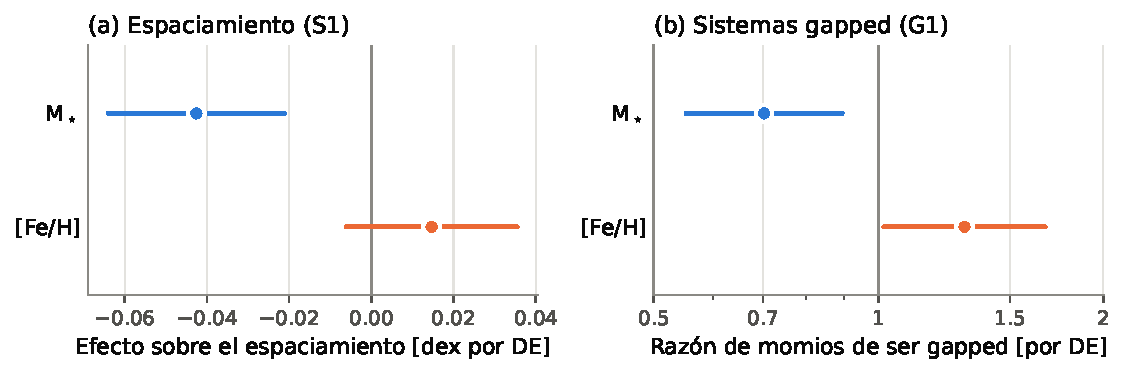
\includegraphics[width=\textwidth]{figuras/A3-F2_efectos_estelares_sobre_la_arquitectura}
\caption{Efecto de la masa estelar y de la metalicidad sobre la arquitectura, por una desviación estándar del predictor: (a) coeficientes del modelo de espaciamiento S1; (b) razones de momios del modelo G1 (escala logarítmica). Las barras son intervalos de confianza al 95\,\%.}
\label{fig:A3-F2}
\end{figure}

\section{Comparación entre los tres análisis}
\label{sec:res-comparacion}

La Tabla~\ref{tab:S-T1} reúne la mejora de cada modelo al incorporar propiedades estelares respecto a su propia base, y la Tabla~\ref{tab:S-T2} resume la dirección e incertidumbre de las asociaciones de masa y metalicidad estelar. Los valores absolutos de AIC, $R^2$ y pseudo-$R^2$ no constituyen una escala compartida entre respuestas y muestras diferentes. Por ello, la comparación se centra en la ganancia dentro de cada análisis y en si se observó también fuera de muestra.

\begin{table}[htbp]
    \centering
    \caption{Contribución de las propiedades estelares en los tres análisis: cambio del modelo estelar respecto al modelo base.}
    \label{tab:S-T1}
    \small
    \resizebox{\textwidth}{!}{%
    \begin{tabular}{lrllrrrr}
    \toprule
    Análisis & $N$ & Modelo base & Modelo estelar & $\Delta$AIC & $\Delta$ajuste & $\Delta$error & $\Delta$error VC \\
    \midrule
    I. Regímenes de radio & 4\,461 & $\log P$ & + $M_\star$ + {[Fe/H]} & -1067.5 & +0.0872 & -0.1214 & -- \\
    I. Super-Tierras y sub-Neptunos & 2\,565 & $\log F$ & + $M_\star$ + {[Fe/H]} + $\log F \times M_\star$ & -376.7 & +0.1176 & -0.0746 & -0.0730 \\
    II. Propiedades físicas & 574 & $s(\log R_p)$ + $\log F$ & + $M_\star$ + {[Fe/H]} & -15.8 & +0.0243 & -0.0063 & -0.0043 \\
    III. Espaciamiento orbital & 615 & $\tilde{R}_p$ + $N_{\rm pl}$ & + $M_\star$ + {[Fe/H]} & -11.3 & +0.0229 & -0.0031 & -- \\
    III. Sistemas \textit{gapped} & 615 & $\tilde{R}_p$ + $N_{\rm pl}$ & + $M_\star$ + {[Fe/H]} & -6.3 & +0.0208 & -0.0084 & -- \\
    \bottomrule
    \end{tabular}
    }
    \par\smallskip
    {\footnotesize\textit{Nota:} $N$ en planetas (análisis I y II) o en sistemas (análisis III). Ajuste: pseudo-$R^2$ de McFadden en los modelos logísticos y $R^2$ en los lineales. Error: log-loss en los modelos logísticos y RMSE en dex en los lineales. Valores negativos de AIC y de las medidas de error indican mejora. VC: validación cruzada agrupada por estrella (solo donde varios planetas comparten estrella).}
\end{table}

\begin{table}[htbp]
    \centering
    \caption{Efecto de un aumento de una desviación estándar de la masa estelar y de la metalicidad en el modelo estelar de cada análisis.}
    \label{tab:S-T2}
    \small
    \resizebox{\textwidth}{!}{%
    \begin{tabular}{llllrrrr}
    \toprule
    Análisis & Respuesta o contraste & Medida & Predictor & Efecto & IC 95\,\% inf. & IC 95\,\% sup. & $p$ \\
    \midrule
    I. Regímenes de radio & Terrestre vs super-Tierra & RRR & $M_\star$ & 0.834 & 0.740 & 0.939 & 0.003 \\
    I. Regímenes de radio & Terrestre vs super-Tierra & RRR & {[Fe/H]} & 0.871 & 0.781 & 0.970 & 0.012 \\
    I. Regímenes de radio & Tipo Neptuno vs super-Tierra & RRR & $M_\star$ & 1.087 & 0.990 & 1.194 & 0.082 \\
    I. Regímenes de radio & Tipo Neptuno vs super-Tierra & RRR & {[Fe/H]} & 1.258 & 1.156 & 1.369 & $<0.001$ \\
    I. Regímenes de radio & Gigante gaseoso vs super-Tierra & RRR & $M_\star$ & 1.860 & 1.645 & 2.104 & $<0.001$ \\
    I. Regímenes de radio & Gigante gaseoso vs super-Tierra & RRR & {[Fe/H]} & 2.146 & 1.915 & 2.405 & $<0.001$ \\
    I. Regímenes de radio & Mayor que Júpiter vs super-Tierra & RRR & $M_\star$ & 8.880 & 7.008 & 11.252 & $<0.001$ \\
    I. Regímenes de radio & Mayor que Júpiter vs super-Tierra & RRR & {[Fe/H]} & 0.885 & 0.717 & 1.093 & 0.258 \\
    I. Super-Tierras y sub-Neptunos & Sub-Neptuno vs super-Tierra & OR & $M_\star$ & 2.671 & 2.334 & 3.057 & $<0.001$ \\
    I. Super-Tierras y sub-Neptunos & Sub-Neptuno vs super-Tierra & OR & {[Fe/H]} & 1.144 & 1.029 & 1.271 & 0.013 \\
    II. Propiedades físicas & $\log M_p$ & coeficiente [dex] & $M_\star$ & 0.076 & 0.031 & 0.121 & $<0.001$ \\
    II. Propiedades físicas & $\log M_p$ & coeficiente [dex] & {[Fe/H]} & 0.030 & -0.008 & 0.068 & 0.125 \\
    III. Espaciamiento orbital & $\log_{10}$ mediana $P_{i+1}/P_i$ & coeficiente [dex] & $M_\star$ & -0.043 & -0.064 & -0.021 & $<0.001$ \\
    III. Espaciamiento orbital & $\log_{10}$ mediana $P_{i+1}/P_i$ & coeficiente [dex] & {[Fe/H]} & 0.015 & -0.006 & 0.035 & 0.166 \\
    III. Sistemas \textit{gapped} & \textit{Gapped} vs no \textit{gapped} & OR & $M_\star$ & 0.703 & 0.552 & 0.894 & 0.004 \\
    III. Sistemas \textit{gapped} & \textit{Gapped} vs no \textit{gapped} & OR & {[Fe/H]} & 1.304 & 1.017 & 1.671 & 0.036 \\
    \bottomrule
    \end{tabular}
    }
    \par\smallskip
    {\footnotesize\textit{Nota:} RRR y OR: 1 indica ausencia de efecto. Coeficientes en dex: 0 indica ausencia de efecto. Intervalos de confianza al 95 \%.}
\end{table}

En los regímenes de radio, la mejora del modelo multinomial fue considerable dentro de la muestra, pero varió entre clases: la masa estelar aportó la mayor reducción del log-loss para cuatro de las cinco, mientras que la metalicidad destacó en los gigantes gaseosos (Figuras~\ref{fig:A1-F2} y~\ref{fig:S-F1}). En el análisis de super-Tierras y sub-Neptunos, tanto la incorporación de las propiedades estelares como la interacción entre flujo y masa estelar mejoraron las métricas de validación cruzada. En la masa de planetas pequeños persistió una mejora fuera de muestra, aunque su magnitud fue modesta. En arquitectura, la masa estelar se asoció con un menor espaciamiento, también en las submuestras de comprobación, mientras que las asociaciones con la condición \textit{gapped} no se sostuvieron en ellas; los modelos conservaron una capacidad explicativa limitada y sus mejoras predictivas no se evaluaron fuera de muestra.

\begin{figure}[htbp]
\centering
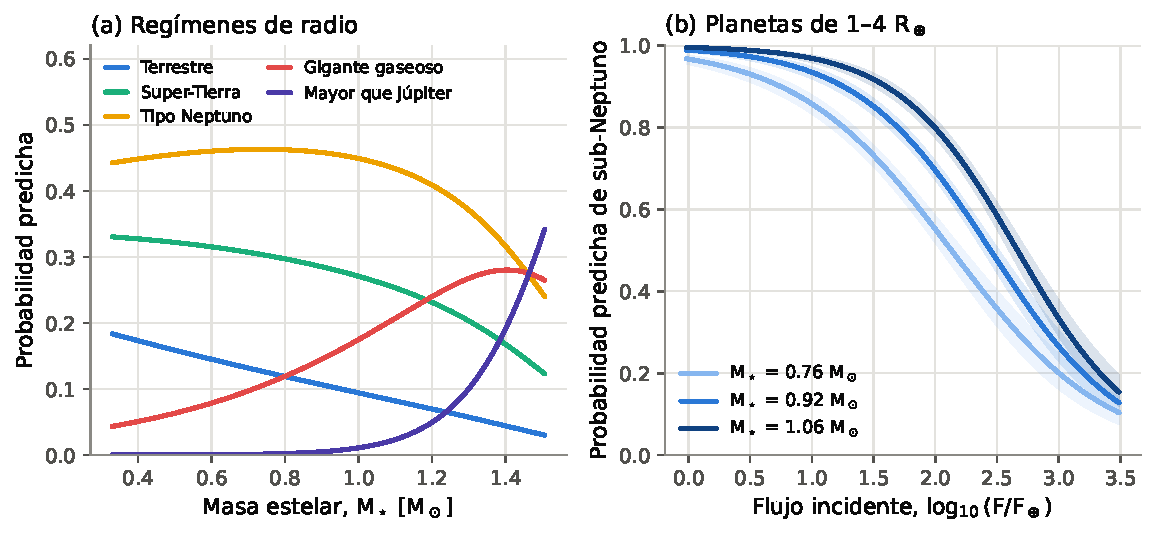
\includegraphics[width=\textwidth]{figuras/S-F1_sintesis_analisis_I}
\caption{Síntesis del análisis~I. (a) Probabilidad predicha de cada régimen de radio en función de la masa estelar (modelo multinomial B1; período y metalicidad en su mediana). (b) Probabilidad predicha de sub-Neptuno en función del flujo incidente para tres masas estelares (modelo $M_2$; bandas: IC del 95\,\%).}
\label{fig:S-F1}
\end{figure}

La Figura~\ref{fig:S-F2} sintetiza las asociaciones estelares estimadas para los tres niveles. En conjunto, los resultados identifican patrones distintos según la propiedad planetaria o del sistema que se tome como respuesta. La comparación muestra dónde se detectó información estelar adicional con los modelos y muestras utilizados; no establece efectos causales ni una clasificación absoluta de los tres niveles mediante una única métrica.

\begin{figure}[htbp]
\centering
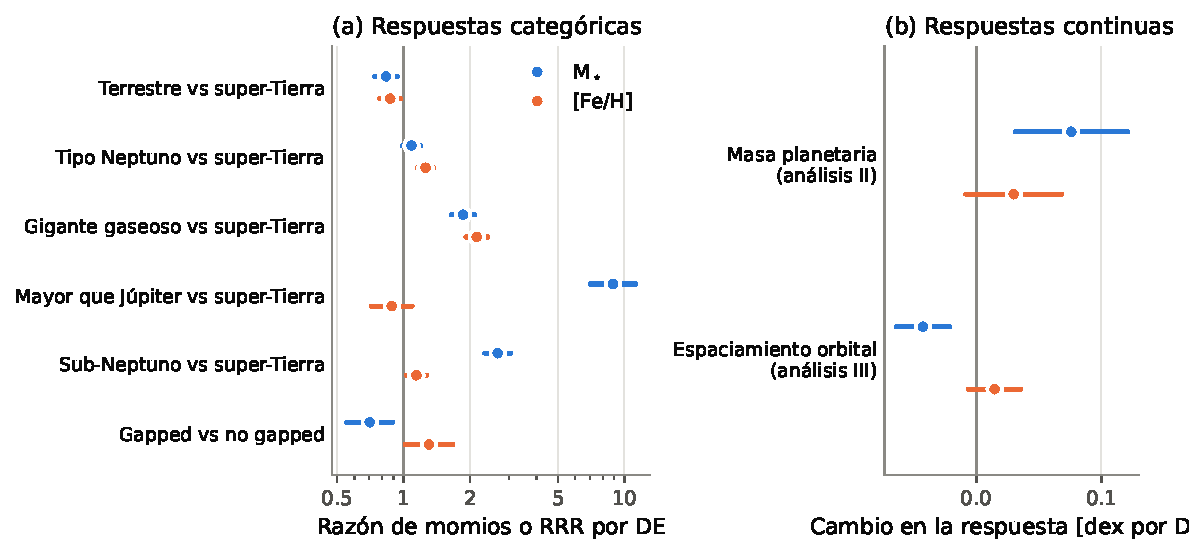
\includegraphics[width=\textwidth]{figuras/S-F2_efectos_estelares_en_los_tres_analisis}
\caption{Efecto de un aumento de una desviación estándar de la masa estelar (azul) y de la metalicidad (naranja) en los modelos estelares de los tres análisis. (a) Razones de momios o de riesgo relativo, en escala logarítmica; (b) coeficientes de los modelos lineales. Las barras son intervalos de confianza al 95\,\%.}
\label{fig:S-F2}
\end{figure}
